\documentclass[11pt]{article}

    \usepackage[breakable]{tcolorbox}
    \usepackage{parskip} % Stop auto-indenting (to mimic markdown behaviour)
    

    % Basic figure setup, for now with no caption control since it's done
    % automatically by Pandoc (which extracts ![](path) syntax from Markdown).
    \usepackage{graphicx}
    % Maintain compatibility with old templates. Remove in nbconvert 6.0
    \let\Oldincludegraphics\includegraphics
    % Ensure that by default, figures have no caption (until we provide a
    % proper Figure object with a Caption API and a way to capture that
    % in the conversion process - todo).
    \usepackage{caption}
    \DeclareCaptionFormat{nocaption}{}
    \captionsetup{format=nocaption,aboveskip=0pt,belowskip=0pt}

    \usepackage{float}
    \floatplacement{figure}{H} % forces figures to be placed at the correct location
    \usepackage{xcolor} % Allow colors to be defined
    \usepackage{enumerate} % Needed for markdown enumerations to work
    \usepackage{geometry} % Used to adjust the document margins
    \usepackage{amsmath} % Equations
    \usepackage{amssymb} % Equations
    \usepackage{textcomp} % defines textquotesingle
    % Hack from http://tex.stackexchange.com/a/47451/13684:
    \AtBeginDocument{%
        \def\PYZsq{\textquotesingle}% Upright quotes in Pygmentized code
    }
    \usepackage{upquote} % Upright quotes for verbatim code
    \usepackage{eurosym} % defines \euro

    \usepackage{iftex}
    \ifPDFTeX
        \usepackage[T1]{fontenc}
        \IfFileExists{alphabeta.sty}{
              \usepackage{alphabeta}
          }{
              \usepackage[mathletters]{ucs}
              \usepackage[utf8x]{inputenc}
          }
    \else
        \usepackage{fontspec}
        \usepackage{unicode-math}
    \fi

    \usepackage{fancyvrb} % verbatim replacement that allows latex
    \usepackage{grffile} % extends the file name processing of package graphics
                         % to support a larger range
    \makeatletter % fix for old versions of grffile with XeLaTeX
    \@ifpackagelater{grffile}{2019/11/01}
    {
      % Do nothing on new versions
    }
    {
      \def\Gread@@xetex#1{%
        \IfFileExists{"\Gin@base".bb}%
        {\Gread@eps{\Gin@base.bb}}%
        {\Gread@@xetex@aux#1}%
      }
    }
    \makeatother
    \usepackage[Export]{adjustbox} % Used to constrain images to a maximum size
    \adjustboxset{max size={0.9\linewidth}{0.9\paperheight}}

    % The hyperref package gives us a pdf with properly built
    % internal navigation ('pdf bookmarks' for the table of contents,
    % internal cross-reference links, web links for URLs, etc.)
    \usepackage{hyperref}
    % The default LaTeX title has an obnoxious amount of whitespace. By default,
    % titling removes some of it. It also provides customization options.
    \usepackage{titling}
    \usepackage{longtable} % longtable support required by pandoc >1.10
    \usepackage{booktabs}  % table support for pandoc > 1.12.2
    \usepackage{array}     % table support for pandoc >= 2.11.3
    \usepackage{calc}      % table minipage width calculation for pandoc >= 2.11.1
    \usepackage[inline]{enumitem} % IRkernel/repr support (it uses the enumerate* environment)
    \usepackage[normalem]{ulem} % ulem is needed to support strikethroughs (\sout)
                                % normalem makes italics be italics, not underlines
    \usepackage{soul}      % strikethrough (\st) support for pandoc >= 3.0.0
    \usepackage{mathrsfs}
    \usepackage{capt-of}
    

    
    % Colors for the hyperref package
    \definecolor{urlcolor}{rgb}{0,.145,.698}
    \definecolor{linkcolor}{rgb}{.71,0.21,0.01}
    \definecolor{citecolor}{rgb}{.12,.54,.11}

    % ANSI colors
    \definecolor{ansi-black}{HTML}{3E424D}
    \definecolor{ansi-black-intense}{HTML}{282C36}
    \definecolor{ansi-red}{HTML}{E75C58}
    \definecolor{ansi-red-intense}{HTML}{B22B31}
    \definecolor{ansi-green}{HTML}{00A250}
    \definecolor{ansi-green-intense}{HTML}{007427}
    \definecolor{ansi-yellow}{HTML}{DDB62B}
    \definecolor{ansi-yellow-intense}{HTML}{B27D12}
    \definecolor{ansi-blue}{HTML}{208FFB}
    \definecolor{ansi-blue-intense}{HTML}{0065CA}
    \definecolor{ansi-magenta}{HTML}{D160C4}
    \definecolor{ansi-magenta-intense}{HTML}{A03196}
    \definecolor{ansi-cyan}{HTML}{60C6C8}
    \definecolor{ansi-cyan-intense}{HTML}{258F8F}
    \definecolor{ansi-white}{HTML}{C5C1B4}
    \definecolor{ansi-white-intense}{HTML}{A1A6B2}
    \definecolor{ansi-default-inverse-fg}{HTML}{FFFFFF}
    \definecolor{ansi-default-inverse-bg}{HTML}{000000}

    % common color for the border for error outputs.
    \definecolor{outerrorbackground}{HTML}{FFDFDF}

    % commands and environments needed by pandoc snippets
    % extracted from the output of `pandoc -s`
    \providecommand{\tightlist}{%
      \setlength{\itemsep}{0pt}\setlength{\parskip}{0pt}}
    \DefineVerbatimEnvironment{Highlighting}{Verbatim}{commandchars=\\\{\}}
    % Add ',fontsize=\small' for more characters per line
    \newenvironment{Shaded}{}{}
    \newcommand{\KeywordTok}[1]{\textcolor[rgb]{0.00,0.44,0.13}{\textbf{{#1}}}}
    \newcommand{\DataTypeTok}[1]{\textcolor[rgb]{0.56,0.13,0.00}{{#1}}}
    \newcommand{\DecValTok}[1]{\textcolor[rgb]{0.25,0.63,0.44}{{#1}}}
    \newcommand{\BaseNTok}[1]{\textcolor[rgb]{0.25,0.63,0.44}{{#1}}}
    \newcommand{\FloatTok}[1]{\textcolor[rgb]{0.25,0.63,0.44}{{#1}}}
    \newcommand{\CharTok}[1]{\textcolor[rgb]{0.25,0.44,0.63}{{#1}}}
    \newcommand{\StringTok}[1]{\textcolor[rgb]{0.25,0.44,0.63}{{#1}}}
    \newcommand{\CommentTok}[1]{\textcolor[rgb]{0.38,0.63,0.69}{\textit{{#1}}}}
    \newcommand{\OtherTok}[1]{\textcolor[rgb]{0.00,0.44,0.13}{{#1}}}
    \newcommand{\AlertTok}[1]{\textcolor[rgb]{1.00,0.00,0.00}{\textbf{{#1}}}}
    \newcommand{\FunctionTok}[1]{\textcolor[rgb]{0.02,0.16,0.49}{{#1}}}
    \newcommand{\RegionMarkerTok}[1]{{#1}}
    \newcommand{\ErrorTok}[1]{\textcolor[rgb]{1.00,0.00,0.00}{\textbf{{#1}}}}
    \newcommand{\NormalTok}[1]{{#1}}

    % Additional commands for more recent versions of Pandoc
    \newcommand{\ConstantTok}[1]{\textcolor[rgb]{0.53,0.00,0.00}{{#1}}}
    \newcommand{\SpecialCharTok}[1]{\textcolor[rgb]{0.25,0.44,0.63}{{#1}}}
    \newcommand{\VerbatimStringTok}[1]{\textcolor[rgb]{0.25,0.44,0.63}{{#1}}}
    \newcommand{\SpecialStringTok}[1]{\textcolor[rgb]{0.73,0.40,0.53}{{#1}}}
    \newcommand{\ImportTok}[1]{{#1}}
    \newcommand{\DocumentationTok}[1]{\textcolor[rgb]{0.73,0.13,0.13}{\textit{{#1}}}}
    \newcommand{\AnnotationTok}[1]{\textcolor[rgb]{0.38,0.63,0.69}{\textbf{\textit{{#1}}}}}
    \newcommand{\CommentVarTok}[1]{\textcolor[rgb]{0.38,0.63,0.69}{\textbf{\textit{{#1}}}}}
    \newcommand{\VariableTok}[1]{\textcolor[rgb]{0.10,0.09,0.49}{{#1}}}
    \newcommand{\ControlFlowTok}[1]{\textcolor[rgb]{0.00,0.44,0.13}{\textbf{{#1}}}}
    \newcommand{\OperatorTok}[1]{\textcolor[rgb]{0.40,0.40,0.40}{{#1}}}
    \newcommand{\BuiltInTok}[1]{{#1}}
    \newcommand{\ExtensionTok}[1]{{#1}}
    \newcommand{\PreprocessorTok}[1]{\textcolor[rgb]{0.74,0.48,0.00}{{#1}}}
    \newcommand{\AttributeTok}[1]{\textcolor[rgb]{0.49,0.56,0.16}{{#1}}}
    \newcommand{\InformationTok}[1]{\textcolor[rgb]{0.38,0.63,0.69}{\textbf{\textit{{#1}}}}}
    \newcommand{\WarningTok}[1]{\textcolor[rgb]{0.38,0.63,0.69}{\textbf{\textit{{#1}}}}}


    % Define a nice break command that doesn't care if a line doesn't already
    % exist.
    \def\br{\hspace*{\fill} \\* }
    % Math Jax compatibility definitions
    \def\gt{>}
    \def\lt{<}
    \let\Oldtex\TeX
    \let\Oldlatex\LaTeX
    \renewcommand{\TeX}{\textrm{\Oldtex}}
    \renewcommand{\LaTeX}{\textrm{\Oldlatex}}
    % Document parameters
    % Document title
    \title{Cartpole}
    \author{Néstor Batista Díaz}
    \date{}
    
    
    
    
    
    
    
% Pygments definitions
\makeatletter
\def\PY@reset{\let\PY@it=\relax \let\PY@bf=\relax%
    \let\PY@ul=\relax \let\PY@tc=\relax%
    \let\PY@bc=\relax \let\PY@ff=\relax}
\def\PY@tok#1{\csname PY@tok@#1\endcsname}
\def\PY@toks#1+{\ifx\relax#1\empty\else%
    \PY@tok{#1}\expandafter\PY@toks\fi}
\def\PY@do#1{\PY@bc{\PY@tc{\PY@ul{%
    \PY@it{\PY@bf{\PY@ff{#1}}}}}}}
\def\PY#1#2{\PY@reset\PY@toks#1+\relax+\PY@do{#2}}

\@namedef{PY@tok@w}{\def\PY@tc##1{\textcolor[rgb]{0.73,0.73,0.73}{##1}}}
\@namedef{PY@tok@c}{\let\PY@it=\textit\def\PY@tc##1{\textcolor[rgb]{0.24,0.48,0.48}{##1}}}
\@namedef{PY@tok@cp}{\def\PY@tc##1{\textcolor[rgb]{0.61,0.40,0.00}{##1}}}
\@namedef{PY@tok@k}{\let\PY@bf=\textbf\def\PY@tc##1{\textcolor[rgb]{0.00,0.50,0.00}{##1}}}
\@namedef{PY@tok@kp}{\def\PY@tc##1{\textcolor[rgb]{0.00,0.50,0.00}{##1}}}
\@namedef{PY@tok@kt}{\def\PY@tc##1{\textcolor[rgb]{0.69,0.00,0.25}{##1}}}
\@namedef{PY@tok@o}{\def\PY@tc##1{\textcolor[rgb]{0.40,0.40,0.40}{##1}}}
\@namedef{PY@tok@ow}{\let\PY@bf=\textbf\def\PY@tc##1{\textcolor[rgb]{0.67,0.13,1.00}{##1}}}
\@namedef{PY@tok@nb}{\def\PY@tc##1{\textcolor[rgb]{0.00,0.50,0.00}{##1}}}
\@namedef{PY@tok@nf}{\def\PY@tc##1{\textcolor[rgb]{0.00,0.00,1.00}{##1}}}
\@namedef{PY@tok@nc}{\let\PY@bf=\textbf\def\PY@tc##1{\textcolor[rgb]{0.00,0.00,1.00}{##1}}}
\@namedef{PY@tok@nn}{\let\PY@bf=\textbf\def\PY@tc##1{\textcolor[rgb]{0.00,0.00,1.00}{##1}}}
\@namedef{PY@tok@ne}{\let\PY@bf=\textbf\def\PY@tc##1{\textcolor[rgb]{0.80,0.25,0.22}{##1}}}
\@namedef{PY@tok@nv}{\def\PY@tc##1{\textcolor[rgb]{0.10,0.09,0.49}{##1}}}
\@namedef{PY@tok@no}{\def\PY@tc##1{\textcolor[rgb]{0.53,0.00,0.00}{##1}}}
\@namedef{PY@tok@nl}{\def\PY@tc##1{\textcolor[rgb]{0.46,0.46,0.00}{##1}}}
\@namedef{PY@tok@ni}{\let\PY@bf=\textbf\def\PY@tc##1{\textcolor[rgb]{0.44,0.44,0.44}{##1}}}
\@namedef{PY@tok@na}{\def\PY@tc##1{\textcolor[rgb]{0.41,0.47,0.13}{##1}}}
\@namedef{PY@tok@nt}{\let\PY@bf=\textbf\def\PY@tc##1{\textcolor[rgb]{0.00,0.50,0.00}{##1}}}
\@namedef{PY@tok@nd}{\def\PY@tc##1{\textcolor[rgb]{0.67,0.13,1.00}{##1}}}
\@namedef{PY@tok@s}{\def\PY@tc##1{\textcolor[rgb]{0.73,0.13,0.13}{##1}}}
\@namedef{PY@tok@sd}{\let\PY@it=\textit\def\PY@tc##1{\textcolor[rgb]{0.73,0.13,0.13}{##1}}}
\@namedef{PY@tok@si}{\let\PY@bf=\textbf\def\PY@tc##1{\textcolor[rgb]{0.64,0.35,0.47}{##1}}}
\@namedef{PY@tok@se}{\let\PY@bf=\textbf\def\PY@tc##1{\textcolor[rgb]{0.67,0.36,0.12}{##1}}}
\@namedef{PY@tok@sr}{\def\PY@tc##1{\textcolor[rgb]{0.64,0.35,0.47}{##1}}}
\@namedef{PY@tok@ss}{\def\PY@tc##1{\textcolor[rgb]{0.10,0.09,0.49}{##1}}}
\@namedef{PY@tok@sx}{\def\PY@tc##1{\textcolor[rgb]{0.00,0.50,0.00}{##1}}}
\@namedef{PY@tok@m}{\def\PY@tc##1{\textcolor[rgb]{0.40,0.40,0.40}{##1}}}
\@namedef{PY@tok@gh}{\let\PY@bf=\textbf\def\PY@tc##1{\textcolor[rgb]{0.00,0.00,0.50}{##1}}}
\@namedef{PY@tok@gu}{\let\PY@bf=\textbf\def\PY@tc##1{\textcolor[rgb]{0.50,0.00,0.50}{##1}}}
\@namedef{PY@tok@gd}{\def\PY@tc##1{\textcolor[rgb]{0.63,0.00,0.00}{##1}}}
\@namedef{PY@tok@gi}{\def\PY@tc##1{\textcolor[rgb]{0.00,0.52,0.00}{##1}}}
\@namedef{PY@tok@gr}{\def\PY@tc##1{\textcolor[rgb]{0.89,0.00,0.00}{##1}}}
\@namedef{PY@tok@ge}{\let\PY@it=\textit}
\@namedef{PY@tok@gs}{\let\PY@bf=\textbf}
\@namedef{PY@tok@ges}{\let\PY@bf=\textbf\let\PY@it=\textit}
\@namedef{PY@tok@gp}{\let\PY@bf=\textbf\def\PY@tc##1{\textcolor[rgb]{0.00,0.00,0.50}{##1}}}
\@namedef{PY@tok@go}{\def\PY@tc##1{\textcolor[rgb]{0.44,0.44,0.44}{##1}}}
\@namedef{PY@tok@gt}{\def\PY@tc##1{\textcolor[rgb]{0.00,0.27,0.87}{##1}}}
\@namedef{PY@tok@err}{\def\PY@bc##1{{\setlength{\fboxsep}{\string -\fboxrule}\fcolorbox[rgb]{1.00,0.00,0.00}{1,1,1}{\strut ##1}}}}
\@namedef{PY@tok@kc}{\let\PY@bf=\textbf\def\PY@tc##1{\textcolor[rgb]{0.00,0.50,0.00}{##1}}}
\@namedef{PY@tok@kd}{\let\PY@bf=\textbf\def\PY@tc##1{\textcolor[rgb]{0.00,0.50,0.00}{##1}}}
\@namedef{PY@tok@kn}{\let\PY@bf=\textbf\def\PY@tc##1{\textcolor[rgb]{0.00,0.50,0.00}{##1}}}
\@namedef{PY@tok@kr}{\let\PY@bf=\textbf\def\PY@tc##1{\textcolor[rgb]{0.00,0.50,0.00}{##1}}}
\@namedef{PY@tok@bp}{\def\PY@tc##1{\textcolor[rgb]{0.00,0.50,0.00}{##1}}}
\@namedef{PY@tok@fm}{\def\PY@tc##1{\textcolor[rgb]{0.00,0.00,1.00}{##1}}}
\@namedef{PY@tok@vc}{\def\PY@tc##1{\textcolor[rgb]{0.10,0.09,0.49}{##1}}}
\@namedef{PY@tok@vg}{\def\PY@tc##1{\textcolor[rgb]{0.10,0.09,0.49}{##1}}}
\@namedef{PY@tok@vi}{\def\PY@tc##1{\textcolor[rgb]{0.10,0.09,0.49}{##1}}}
\@namedef{PY@tok@vm}{\def\PY@tc##1{\textcolor[rgb]{0.10,0.09,0.49}{##1}}}
\@namedef{PY@tok@sa}{\def\PY@tc##1{\textcolor[rgb]{0.73,0.13,0.13}{##1}}}
\@namedef{PY@tok@sb}{\def\PY@tc##1{\textcolor[rgb]{0.73,0.13,0.13}{##1}}}
\@namedef{PY@tok@sc}{\def\PY@tc##1{\textcolor[rgb]{0.73,0.13,0.13}{##1}}}
\@namedef{PY@tok@dl}{\def\PY@tc##1{\textcolor[rgb]{0.73,0.13,0.13}{##1}}}
\@namedef{PY@tok@s2}{\def\PY@tc##1{\textcolor[rgb]{0.73,0.13,0.13}{##1}}}
\@namedef{PY@tok@sh}{\def\PY@tc##1{\textcolor[rgb]{0.73,0.13,0.13}{##1}}}
\@namedef{PY@tok@s1}{\def\PY@tc##1{\textcolor[rgb]{0.73,0.13,0.13}{##1}}}
\@namedef{PY@tok@mb}{\def\PY@tc##1{\textcolor[rgb]{0.40,0.40,0.40}{##1}}}
\@namedef{PY@tok@mf}{\def\PY@tc##1{\textcolor[rgb]{0.40,0.40,0.40}{##1}}}
\@namedef{PY@tok@mh}{\def\PY@tc##1{\textcolor[rgb]{0.40,0.40,0.40}{##1}}}
\@namedef{PY@tok@mi}{\def\PY@tc##1{\textcolor[rgb]{0.40,0.40,0.40}{##1}}}
\@namedef{PY@tok@il}{\def\PY@tc##1{\textcolor[rgb]{0.40,0.40,0.40}{##1}}}
\@namedef{PY@tok@mo}{\def\PY@tc##1{\textcolor[rgb]{0.40,0.40,0.40}{##1}}}
\@namedef{PY@tok@ch}{\let\PY@it=\textit\def\PY@tc##1{\textcolor[rgb]{0.24,0.48,0.48}{##1}}}
\@namedef{PY@tok@cm}{\let\PY@it=\textit\def\PY@tc##1{\textcolor[rgb]{0.24,0.48,0.48}{##1}}}
\@namedef{PY@tok@cpf}{\let\PY@it=\textit\def\PY@tc##1{\textcolor[rgb]{0.24,0.48,0.48}{##1}}}
\@namedef{PY@tok@c1}{\let\PY@it=\textit\def\PY@tc##1{\textcolor[rgb]{0.24,0.48,0.48}{##1}}}
\@namedef{PY@tok@cs}{\let\PY@it=\textit\def\PY@tc##1{\textcolor[rgb]{0.24,0.48,0.48}{##1}}}

\def\PYZbs{\char`\\}
\def\PYZus{\char`\_}
\def\PYZob{\char`\{}
\def\PYZcb{\char`\}}
\def\PYZca{\char`\^}
\def\PYZam{\char`\&}
\def\PYZlt{\char`\<}
\def\PYZgt{\char`\>}
\def\PYZsh{\char`\#}
\def\PYZpc{\char`\%}
\def\PYZdl{\char`\$}
\def\PYZhy{\char`\-}
\def\PYZsq{\char`\'}
\def\PYZdq{\char`\"}
\def\PYZti{\char`\~}
% for compatibility with earlier versions
\def\PYZat{@}
\def\PYZlb{[}
\def\PYZrb{]}
\makeatother


    % For linebreaks inside Verbatim environment from package fancyvrb.
    \makeatletter
        \newbox\Wrappedcontinuationbox
        \newbox\Wrappedvisiblespacebox
        \newcommand*\Wrappedvisiblespace {\textcolor{red}{\textvisiblespace}}
        \newcommand*\Wrappedcontinuationsymbol {\textcolor{red}{\llap{\tiny$\m@th\hookrightarrow$}}}
        \newcommand*\Wrappedcontinuationindent {3ex }
        \newcommand*\Wrappedafterbreak {\kern\Wrappedcontinuationindent\copy\Wrappedcontinuationbox}
        % Take advantage of the already applied Pygments mark-up to insert
        % potential linebreaks for TeX processing.
        %        {, <, #, %, $, ' and ": go to next line.
        %        _, }, ^, &, >, - and ~: stay at end of broken line.
        % Use of \textquotesingle for straight quote.
        \newcommand*\Wrappedbreaksatspecials {%
            \def\PYGZus{\discretionary{\char`\_}{\Wrappedafterbreak}{\char`\_}}%
            \def\PYGZob{\discretionary{}{\Wrappedafterbreak\char`\{}{\char`\{}}%
            \def\PYGZcb{\discretionary{\char`\}}{\Wrappedafterbreak}{\char`\}}}%
            \def\PYGZca{\discretionary{\char`\^}{\Wrappedafterbreak}{\char`\^}}%
            \def\PYGZam{\discretionary{\char`\&}{\Wrappedafterbreak}{\char`\&}}%
            \def\PYGZlt{\discretionary{}{\Wrappedafterbreak\char`\<}{\char`\<}}%
            \def\PYGZgt{\discretionary{\char`\>}{\Wrappedafterbreak}{\char`\>}}%
            \def\PYGZsh{\discretionary{}{\Wrappedafterbreak\char`\#}{\char`\#}}%
            \def\PYGZpc{\discretionary{}{\Wrappedafterbreak\char`\%}{\char`\%}}%
            \def\PYGZdl{\discretionary{}{\Wrappedafterbreak\char`\$}{\char`\$}}%
            \def\PYGZhy{\discretionary{\char`\-}{\Wrappedafterbreak}{\char`\-}}%
            \def\PYGZsq{\discretionary{}{\Wrappedafterbreak\textquotesingle}{\textquotesingle}}%
            \def\PYGZdq{\discretionary{}{\Wrappedafterbreak\char`\"}{\char`\"}}%
            \def\PYGZti{\discretionary{\char`\~}{\Wrappedafterbreak}{\char`\~}}%
        }
        % Some characters . , ; ? ! / are not pygmentized.
        % This macro makes them "active" and they will insert potential linebreaks
        \newcommand*\Wrappedbreaksatpunct {%
            \lccode`\~`\.\lowercase{\def~}{\discretionary{\hbox{\char`\.}}{\Wrappedafterbreak}{\hbox{\char`\.}}}%
            \lccode`\~`\,\lowercase{\def~}{\discretionary{\hbox{\char`\,}}{\Wrappedafterbreak}{\hbox{\char`\,}}}%
            \lccode`\~`\;\lowercase{\def~}{\discretionary{\hbox{\char`\;}}{\Wrappedafterbreak}{\hbox{\char`\;}}}%
            \lccode`\~`\:\lowercase{\def~}{\discretionary{\hbox{\char`\:}}{\Wrappedafterbreak}{\hbox{\char`\:}}}%
            \lccode`\~`\?\lowercase{\def~}{\discretionary{\hbox{\char`\?}}{\Wrappedafterbreak}{\hbox{\char`\?}}}%
            \lccode`\~`\!\lowercase{\def~}{\discretionary{\hbox{\char`\!}}{\Wrappedafterbreak}{\hbox{\char`\!}}}%
            \lccode`\~`\/\lowercase{\def~}{\discretionary{\hbox{\char`\/}}{\Wrappedafterbreak}{\hbox{\char`\/}}}%
            \catcode`\.\active
            \catcode`\,\active
            \catcode`\;\active
            \catcode`\:\active
            \catcode`\?\active
            \catcode`\!\active
            \catcode`\/\active
            \lccode`\~`\~
        }
    \makeatother

    \let\OriginalVerbatim=\Verbatim
    \makeatletter
    \renewcommand{\Verbatim}[1][1]{%
        %\parskip\z@skip
        \sbox\Wrappedcontinuationbox {\Wrappedcontinuationsymbol}%
        \sbox\Wrappedvisiblespacebox {\FV@SetupFont\Wrappedvisiblespace}%
        \def\FancyVerbFormatLine ##1{\hsize\linewidth
            \vtop{\raggedright\hyphenpenalty\z@\exhyphenpenalty\z@
                \doublehyphendemerits\z@\finalhyphendemerits\z@
                \strut ##1\strut}%
        }%
        % If the linebreak is at a space, the latter will be displayed as visible
        % space at end of first line, and a continuation symbol starts next line.
        % Stretch/shrink are however usually zero for typewriter font.
        \def\FV@Space {%
            \nobreak\hskip\z@ plus\fontdimen3\font minus\fontdimen4\font
            \discretionary{\copy\Wrappedvisiblespacebox}{\Wrappedafterbreak}
            {\kern\fontdimen2\font}%
        }%

        % Allow breaks at special characters using \PYG... macros.
        \Wrappedbreaksatspecials
        % Breaks at punctuation characters . , ; ? ! and / need catcode=\active
        \OriginalVerbatim[#1,codes*=\Wrappedbreaksatpunct]%
    }
    \makeatother

    % Exact colors from NB
    \definecolor{incolor}{HTML}{303F9F}
    \definecolor{outcolor}{HTML}{D84315}
    \definecolor{cellborder}{HTML}{CFCFCF}
    \definecolor{cellbackground}{HTML}{F7F7F7}

    % prompt
    \makeatletter
    \newcommand{\boxspacing}{\kern\kvtcb@left@rule\kern\kvtcb@boxsep}
    \makeatother
    \newcommand{\prompt}[4]{
        {\ttfamily\llap{{\color{#2}[#3]:\hspace{3pt}#4}}\vspace{-\baselineskip}}
    }
    

    
    % Prevent overflowing lines due to hard-to-break entities
    \sloppy
    % Setup hyperref package
    \hypersetup{
      breaklinks=true,  % so long urls are correctly broken across lines
      colorlinks=true,
      urlcolor=urlcolor,
      linkcolor=linkcolor,
      citecolor=citecolor,
      }
    % Slightly bigger margins than the latex defaults
    
    \geometry{verbose,tmargin=1in,bmargin=1in,lmargin=1in,rmargin=1in}
    
    

\begin{document}
    
    \maketitle
    
    

    
    \begin{tcolorbox}[breakable, size=fbox, boxrule=1pt, pad at break*=1mm,colback=white, colframe=black]
\prompt{In}{incolor}{6}{\boxspacing}
\begin{Verbatim}[commandchars=\\\{\}]
\PY{c+c1}{\PYZsh{} This Python 3 environment comes with many helpful analytics libraries installed}
\PY{c+c1}{\PYZsh{} It is defined by the kaggle/python docker image: https://github.com/kaggle/docker\PYZhy{}python}
\PY{c+c1}{\PYZsh{} For example, here\PYZsq{}s several helpful packages to load in }

\PY{k+kn}{import} \PY{n+nn}{numpy} \PY{k}{as} \PY{n+nn}{np} \PY{c+c1}{\PYZsh{} linear algebra}
\PY{k+kn}{import} \PY{n+nn}{pandas} \PY{k}{as} \PY{n+nn}{pd} \PY{c+c1}{\PYZsh{} data processing, CSV file I/O (e.g. pd.read\PYZus{}csv)}
\PY{k+kn}{import} \PY{n+nn}{gym} \PY{c+c1}{\PYZsh{} for environment}
\PY{k+kn}{from} \PY{n+nn}{collections} \PY{k+kn}{import} \PY{n}{deque}
\PY{k+kn}{from} \PY{n+nn}{keras}\PY{n+nn}{.}\PY{n+nn}{models} \PY{k+kn}{import} \PY{n}{Sequential}
\PY{k+kn}{from} \PY{n+nn}{keras}\PY{n+nn}{.}\PY{n+nn}{layers} \PY{k+kn}{import} \PY{n}{Dense}
\PY{k+kn}{from} \PY{n+nn}{keras}\PY{n+nn}{.}\PY{n+nn}{optimizers} \PY{k+kn}{import} \PY{n}{Adam} \PY{c+c1}{\PYZsh{} adaptive momentum }
\PY{k+kn}{from} \PY{n+nn}{keras}\PY{n+nn}{.}\PY{n+nn}{callbacks} \PY{k+kn}{import} \PY{n}{TensorBoard}
\PY{k+kn}{import} \PY{n+nn}{random}
\PY{k+kn}{import} \PY{n+nn}{webbrowser}

\PY{c+c1}{\PYZsh{} Input data files are available in the \PYZdq{}../input/\PYZdq{} directory.}
\PY{c+c1}{\PYZsh{} For example, running this (by clicking run or pressing Shift+Enter) will list all files under the input directory}
\end{Verbatim}
\end{tcolorbox}

    \begin{tcolorbox}[breakable, size=fbox, boxrule=1pt, pad at break*=1mm,colback=white, colframe=black]
\prompt{In}{incolor}{7}{\boxspacing}
\begin{Verbatim}[commandchars=\\\{\}]
\PY{c+c1}{\PYZsh{} Registra métricas de entrenamiento en TensorBoard para visualización y depuración}
\PY{n}{tensorboard\PYZus{}callback} \PY{o}{=} \PY{n}{TensorBoard}\PY{p}{(}\PY{n}{log\PYZus{}dir} \PY{o}{=} \PY{l+s+s2}{\PYZdq{}}\PY{l+s+s2}{./logs}\PY{l+s+s2}{\PYZdq{}}\PY{p}{)}
\end{Verbatim}
\end{tcolorbox}

    \begin{tcolorbox}[breakable, size=fbox, boxrule=1pt, pad at break*=1mm,colback=white, colframe=black]
\prompt{In}{incolor}{8}{\boxspacing}
\begin{Verbatim}[commandchars=\\\{\}]
\PY{k}{class} \PY{n+nc}{DQLAgent}\PY{p}{(}\PY{p}{)}\PY{p}{:} 
    
    \PY{k}{def} \PY{n+nf+fm}{\PYZus{}\PYZus{}init\PYZus{}\PYZus{}}\PY{p}{(}\PY{n+nb+bp}{self}\PY{p}{,} \PY{n}{env}\PY{p}{)}\PY{p}{:}
        \PY{c+c1}{\PYZsh{} parameters and hyperparameters}
        
        \PY{c+c1}{\PYZsh{} this part is for neural network or build\PYZus{}model()}
        \PY{n+nb+bp}{self}\PY{o}{.}\PY{n}{state\PYZus{}size} \PY{o}{=} \PY{n}{env}\PY{o}{.}\PY{n}{observation\PYZus{}space}\PY{o}{.}\PY{n}{shape}\PY{p}{[}\PY{l+m+mi}{0}\PY{p}{]} \PY{c+c1}{\PYZsh{} this is for input of neural network node size}
        \PY{n+nb+bp}{self}\PY{o}{.}\PY{n}{action\PYZus{}size} \PY{o}{=} \PY{n}{env}\PY{o}{.}\PY{n}{action\PYZus{}space}\PY{o}{.}\PY{n}{n} \PY{c+c1}{\PYZsh{} this is for out of neural network node size}
        
        \PY{c+c1}{\PYZsh{} this part is for replay()}
        \PY{n+nb+bp}{self}\PY{o}{.}\PY{n}{gamma} \PY{o}{=} \PY{l+m+mf}{0.95}
        \PY{n+nb+bp}{self}\PY{o}{.}\PY{n}{learning\PYZus{}rate} \PY{o}{=} \PY{l+m+mf}{0.001}
        
        \PY{c+c1}{\PYZsh{} this part is for adaptiveEGreedy()}
        \PY{n+nb+bp}{self}\PY{o}{.}\PY{n}{epsilon} \PY{o}{=} \PY{l+m+mi}{1} \PY{c+c1}{\PYZsh{} initial exploration rate}
        \PY{n+nb+bp}{self}\PY{o}{.}\PY{n}{epsilon\PYZus{}decay} \PY{o}{=} \PY{l+m+mf}{0.995}
        \PY{n+nb+bp}{self}\PY{o}{.}\PY{n}{epsilon\PYZus{}min} \PY{o}{=} \PY{l+m+mf}{0.01}
        
        \PY{n+nb+bp}{self}\PY{o}{.}\PY{n}{memory} \PY{o}{=} \PY{n}{deque}\PY{p}{(}\PY{n}{maxlen} \PY{o}{=} \PY{l+m+mi}{1000}\PY{p}{)} \PY{c+c1}{\PYZsh{} a list with 1000 memory, if it becomes full first inputs will be deleted}
        
        \PY{n+nb+bp}{self}\PY{o}{.}\PY{n}{model} \PY{o}{=} \PY{n+nb+bp}{self}\PY{o}{.}\PY{n}{build\PYZus{}model}\PY{p}{(}\PY{p}{)}
    
    \PY{k}{def} \PY{n+nf}{build\PYZus{}model}\PY{p}{(}\PY{n+nb+bp}{self}\PY{p}{)}\PY{p}{:}
        \PY{c+c1}{\PYZsh{} neural network for deep Q learning}
        \PY{n}{model} \PY{o}{=} \PY{n}{Sequential}\PY{p}{(}\PY{p}{)}
        \PY{n}{model}\PY{o}{.}\PY{n}{add}\PY{p}{(}\PY{n}{Dense}\PY{p}{(}\PY{l+m+mi}{48}\PY{p}{,} \PY{n}{input\PYZus{}dim} \PY{o}{=} \PY{n+nb+bp}{self}\PY{o}{.}\PY{n}{state\PYZus{}size}\PY{p}{,} \PY{n}{activation} \PY{o}{=} \PY{l+s+s1}{\PYZsq{}}\PY{l+s+s1}{tanh}\PY{l+s+s1}{\PYZsq{}}\PY{p}{)}\PY{p}{)} \PY{c+c1}{\PYZsh{} first hidden layer}
        \PY{n}{model}\PY{o}{.}\PY{n}{add}\PY{p}{(}\PY{n}{Dense}\PY{p}{(}\PY{n+nb+bp}{self}\PY{o}{.}\PY{n}{action\PYZus{}size}\PY{p}{,} \PY{n}{activation} \PY{o}{=} \PY{l+s+s1}{\PYZsq{}}\PY{l+s+s1}{linear}\PY{l+s+s1}{\PYZsq{}}\PY{p}{)}\PY{p}{)} \PY{c+c1}{\PYZsh{} output layer}
        \PY{n}{model}\PY{o}{.}\PY{n}{compile}\PY{p}{(}\PY{n}{loss} \PY{o}{=} \PY{l+s+s1}{\PYZsq{}}\PY{l+s+s1}{mse}\PY{l+s+s1}{\PYZsq{}}\PY{p}{,} \PY{n}{optimizer} \PY{o}{=} \PY{n}{Adam}\PY{p}{(}\PY{n}{learning\PYZus{}rate} \PY{o}{=} \PY{n+nb+bp}{self}\PY{o}{.}\PY{n}{learning\PYZus{}rate}\PY{p}{)}\PY{p}{)}
        \PY{k}{return} \PY{n}{model}
    
    \PY{k}{def} \PY{n+nf}{remember}\PY{p}{(}\PY{n+nb+bp}{self}\PY{p}{,} \PY{n}{state}\PY{p}{,} \PY{n}{action}\PY{p}{,} \PY{n}{reward}\PY{p}{,} \PY{n}{next\PYZus{}state}\PY{p}{,} \PY{n}{done}\PY{p}{)}\PY{p}{:}
        \PY{c+c1}{\PYZsh{} storage}
        \PY{n+nb+bp}{self}\PY{o}{.}\PY{n}{memory}\PY{o}{.}\PY{n}{append}\PY{p}{(}\PY{p}{(}\PY{n}{state}\PY{p}{,} \PY{n}{action}\PY{p}{,} \PY{n}{reward}\PY{p}{,} \PY{n}{next\PYZus{}state}\PY{p}{,} \PY{n}{done}\PY{p}{)}\PY{p}{)}
    
    \PY{k}{def} \PY{n+nf}{act}\PY{p}{(}\PY{n+nb+bp}{self}\PY{p}{,} \PY{n}{state}\PY{p}{)}\PY{p}{:}
        \PY{c+c1}{\PYZsh{} acting, exploit or explore}
        \PY{k}{if} \PY{n}{random}\PY{o}{.}\PY{n}{uniform}\PY{p}{(}\PY{l+m+mi}{0}\PY{p}{,}\PY{l+m+mi}{1}\PY{p}{)} \PY{o}{\PYZlt{}}\PY{o}{=} \PY{n+nb+bp}{self}\PY{o}{.}\PY{n}{epsilon}\PY{p}{:}
            \PY{k}{return} \PY{n}{env}\PY{o}{.}\PY{n}{action\PYZus{}space}\PY{o}{.}\PY{n}{sample}\PY{p}{(}\PY{p}{)}
        \PY{k}{else}\PY{p}{:}
            \PY{n}{act\PYZus{}values} \PY{o}{=} \PY{n+nb+bp}{self}\PY{o}{.}\PY{n}{model}\PY{o}{.}\PY{n}{predict}\PY{p}{(}\PY{n}{state}\PY{p}{)}
            \PY{k}{return} \PY{n}{np}\PY{o}{.}\PY{n}{argmax}\PY{p}{(}\PY{n}{act\PYZus{}values}\PY{p}{[}\PY{l+m+mi}{0}\PY{p}{]}\PY{p}{)}
            
    
    \PY{k}{def} \PY{n+nf}{replay}\PY{p}{(}\PY{n+nb+bp}{self}\PY{p}{,} \PY{n}{batch\PYZus{}size}\PY{p}{)}\PY{p}{:}
        \PY{c+c1}{\PYZsh{} training}
        
        \PY{k}{if} \PY{n+nb}{len}\PY{p}{(}\PY{n+nb+bp}{self}\PY{o}{.}\PY{n}{memory}\PY{p}{)} \PY{o}{\PYZlt{}} \PY{n}{batch\PYZus{}size}\PY{p}{:}
            \PY{k}{return} \PY{c+c1}{\PYZsh{} memory is still not full}
        
        \PY{n}{minibatch} \PY{o}{=} \PY{n}{random}\PY{o}{.}\PY{n}{sample}\PY{p}{(}\PY{n+nb+bp}{self}\PY{o}{.}\PY{n}{memory}\PY{p}{,} \PY{n}{batch\PYZus{}size}\PY{p}{)} \PY{c+c1}{\PYZsh{} take 16 (batch\PYZus{}size) random samples from memory}
        \PY{k}{for} \PY{n}{state}\PY{p}{,} \PY{n}{action}\PY{p}{,} \PY{n}{reward}\PY{p}{,} \PY{n}{next\PYZus{}state}\PY{p}{,} \PY{n}{done} \PY{o+ow}{in} \PY{n}{minibatch}\PY{p}{:}
            \PY{k}{if} \PY{n}{done}\PY{p}{:} \PY{c+c1}{\PYZsh{} if the game is over, I dont have next state, I just have reward }
                \PY{n}{target} \PY{o}{=} \PY{n}{reward}
            \PY{k}{else}\PY{p}{:}
                \PY{n}{target} \PY{o}{=} \PY{n}{reward} \PY{o}{+} \PY{n+nb+bp}{self}\PY{o}{.}\PY{n}{gamma} \PY{o}{*} \PY{n}{np}\PY{o}{.}\PY{n}{amax}\PY{p}{(}\PY{n+nb+bp}{self}\PY{o}{.}\PY{n}{model}\PY{o}{.}\PY{n}{predict}\PY{p}{(}\PY{n}{next\PYZus{}state}\PY{p}{)}\PY{p}{[}\PY{l+m+mi}{0}\PY{p}{]}\PY{p}{)} 
                \PY{c+c1}{\PYZsh{} target = R(s,a) + gamma * max Q`(s`,a`)}
                \PY{c+c1}{\PYZsh{} target (max Q` value) is output of Neural Network which takes s` as an input }
                \PY{c+c1}{\PYZsh{} amax(): flatten the lists (make them 1 list) and take max value}
            \PY{n}{train\PYZus{}target} \PY{o}{=} \PY{n+nb+bp}{self}\PY{o}{.}\PY{n}{model}\PY{o}{.}\PY{n}{predict}\PY{p}{(}\PY{n}{state}\PY{p}{)} \PY{c+c1}{\PYZsh{} s \PYZhy{}\PYZhy{}\PYZgt{} NN \PYZhy{}\PYZhy{}\PYZgt{} Q(s,a)=train\PYZus{}target}
            \PY{n}{train\PYZus{}target}\PY{p}{[}\PY{l+m+mi}{0}\PY{p}{]}\PY{p}{[}\PY{n}{action}\PY{p}{]} \PY{o}{=} \PY{n}{target}
            \PY{n+nb+bp}{self}\PY{o}{.}\PY{n}{model}\PY{o}{.}\PY{n}{fit}\PY{p}{(}\PY{n}{state}\PY{p}{,} \PY{n}{train\PYZus{}target}\PY{p}{,} \PY{n}{verbose} \PY{o}{=} \PY{l+m+mi}{0}\PY{p}{,} \PY{n}{callbacks}\PY{o}{=}\PY{p}{[}\PY{n}{tensorboard\PYZus{}callback}\PY{p}{]}\PY{p}{)} \PY{c+c1}{\PYZsh{} verbose: dont show loss and epoch}
    
    \PY{k}{def} \PY{n+nf}{adaptiveEGreedy}\PY{p}{(}\PY{n+nb+bp}{self}\PY{p}{)}\PY{p}{:}
        \PY{k}{if} \PY{n+nb+bp}{self}\PY{o}{.}\PY{n}{epsilon} \PY{o}{\PYZgt{}} \PY{n+nb+bp}{self}\PY{o}{.}\PY{n}{epsilon\PYZus{}min}\PY{p}{:}
            \PY{n+nb+bp}{self}\PY{o}{.}\PY{n}{epsilon} \PY{o}{*}\PY{o}{=} \PY{n+nb+bp}{self}\PY{o}{.}\PY{n}{epsilon\PYZus{}decay}
            

\PY{k}{if} \PY{n+nv+vm}{\PYZus{}\PYZus{}name\PYZus{}\PYZus{}} \PY{o}{==} \PY{l+s+s2}{\PYZdq{}}\PY{l+s+s2}{\PYZus{}\PYZus{}main\PYZus{}\PYZus{}}\PY{l+s+s2}{\PYZdq{}}\PY{p}{:}
    
    \PY{c+c1}{\PYZsh{} initialize gym environment and agent}
    \PY{n}{env} \PY{o}{=} \PY{n}{gym}\PY{o}{.}\PY{n}{make}\PY{p}{(}\PY{l+s+s1}{\PYZsq{}}\PY{l+s+s1}{CartPole\PYZhy{}v0}\PY{l+s+s1}{\PYZsq{}}\PY{p}{)}
    \PY{n}{agent} \PY{o}{=} \PY{n}{DQLAgent}\PY{p}{(}\PY{n}{env}\PY{p}{)}

    \PY{n}{batch\PYZus{}size} \PY{o}{=} \PY{l+m+mi}{16}
    \PY{n}{episodes} \PY{o}{=} \PY{l+m+mi}{10}
    \PY{k}{for} \PY{n}{e} \PY{o+ow}{in} \PY{n+nb}{range}\PY{p}{(}\PY{n}{episodes}\PY{p}{)}\PY{p}{:}
        
        \PY{c+c1}{\PYZsh{} initialize environment}
        \PY{n}{state} \PY{o}{=} \PY{n}{env}\PY{o}{.}\PY{n}{reset}\PY{p}{(}\PY{p}{)}
        \PY{n}{state} \PY{o}{=} \PY{n}{np}\PY{o}{.}\PY{n}{reshape}\PY{p}{(}\PY{n}{state}\PY{p}{[}\PY{l+m+mi}{0}\PY{p}{]}\PY{p}{,} \PY{p}{[}\PY{l+m+mi}{1}\PY{p}{,}\PY{l+m+mi}{4}\PY{p}{]}\PY{p}{)}
        
        \PY{n}{time} \PY{o}{=} \PY{l+m+mi}{0} \PY{c+c1}{\PYZsh{} each second I will get reward, because I want to sustain a balance forever}
        \PY{k}{while} \PY{k+kc}{True}\PY{p}{:}
            
            \PY{c+c1}{\PYZsh{} act}
            \PY{n}{action} \PY{o}{=} \PY{n}{agent}\PY{o}{.}\PY{n}{act}\PY{p}{(}\PY{n}{state}\PY{p}{)}
            
            \PY{c+c1}{\PYZsh{} step}
            \PY{n}{next\PYZus{}state}\PY{p}{,} \PY{n}{reward}\PY{p}{,} \PY{n}{done}\PY{p}{,} \PY{n}{\PYZus{}} \PY{p}{,} \PY{n}{\PYZus{}}\PY{o}{=} \PY{n}{env}\PY{o}{.}\PY{n}{step}\PY{p}{(}\PY{n}{action}\PY{p}{)}
            \PY{n}{next\PYZus{}state} \PY{o}{=} \PY{n}{np}\PY{o}{.}\PY{n}{reshape}\PY{p}{(}\PY{n}{next\PYZus{}state}\PY{p}{,} \PY{p}{[}\PY{l+m+mi}{1}\PY{p}{,}\PY{l+m+mi}{4}\PY{p}{]}\PY{p}{)}
            
            \PY{c+c1}{\PYZsh{} remember / storage}
            \PY{n}{agent}\PY{o}{.}\PY{n}{remember}\PY{p}{(}\PY{n}{state}\PY{p}{,} \PY{n}{action}\PY{p}{,} \PY{n}{reward}\PY{p}{,} \PY{n}{next\PYZus{}state}\PY{p}{,} \PY{n}{done}\PY{p}{)}
            
            \PY{c+c1}{\PYZsh{} update state}
            \PY{n}{state} \PY{o}{=} \PY{n}{next\PYZus{}state}
            
            \PY{c+c1}{\PYZsh{} replay}
            \PY{n}{agent}\PY{o}{.}\PY{n}{replay}\PY{p}{(}\PY{n}{batch\PYZus{}size}\PY{p}{)}
            
            \PY{c+c1}{\PYZsh{} adjust epsilon}
            \PY{n}{agent}\PY{o}{.}\PY{n}{adaptiveEGreedy}\PY{p}{(}\PY{p}{)}

            \PY{c+c1}{\PYZsh{} Creamos un condicional random para guardar el modelo de vez en cuando}
            \PY{k}{if}\PY{p}{(}\PY{n}{random}\PY{o}{.}\PY{n}{random}\PY{p}{(}\PY{p}{)} \PY{o}{\PYZlt{}} \PY{l+m+mf}{0.1}\PY{p}{)}\PY{p}{:}
                \PY{n}{agent}\PY{o}{.}\PY{n}{model}\PY{o}{.}\PY{n}{save}\PY{p}{(}\PY{l+s+s1}{\PYZsq{}}\PY{l+s+s1}{cartpole\PYZus{}pruebas.keras}\PY{l+s+s1}{\PYZsq{}}\PY{p}{)}
                \PY{n+nb}{print}\PY{p}{(}\PY{l+s+s2}{\PYZdq{}}\PY{l+s+s2}{Model Saved}\PY{l+s+s2}{\PYZdq{}}\PY{p}{)}
            
            \PY{n}{time} \PY{o}{+}\PY{o}{=} \PY{l+m+mi}{1}
            
            \PY{k}{if} \PY{n}{done}\PY{p}{:}
                \PY{n+nb}{print}\PY{p}{(}\PY{l+s+s1}{\PYZsq{}}\PY{l+s+s1}{episode: }\PY{l+s+si}{\PYZob{}\PYZcb{}}\PY{l+s+s1}{, time: }\PY{l+s+si}{\PYZob{}\PYZcb{}}\PY{l+s+s1}{\PYZsq{}}\PY{o}{.}\PY{n}{format}\PY{p}{(}\PY{n}{e}\PY{p}{,} \PY{n}{time}\PY{p}{)}\PY{p}{)}
                \PY{k}{break}
    \PY{c+c1}{\PYZsh{} Guardamos el modelo entrenado        }
    \PY{n}{agent}\PY{o}{.}\PY{n}{model}\PY{o}{.}\PY{n}{save}\PY{p}{(}\PY{l+s+s1}{\PYZsq{}}\PY{l+s+s1}{cartpole\PYZus{}pruebas.keras}\PY{l+s+s1}{\PYZsq{}}\PY{p}{)}
    \PY{n+nb}{print}\PY{p}{(}\PY{l+s+s2}{\PYZdq{}}\PY{l+s+s2}{Model Saved}\PY{l+s+s2}{\PYZdq{}}\PY{p}{)}
\end{Verbatim}
\end{tcolorbox}

\begin{tcolorbox}[breakable, size=fbox, boxrule=1pt, pad at break*=1mm,colback=cellbackground, colframe=cellborder]
    \prompt{Out}{outcolor}{8}{\boxspacing}
    \begin{Verbatim}[commandchars=\\\{\}]
episode: 0, time: 12
\textbf{1/1} \textcolor{ansi-green}{-----------------------} \textbf{0s} 44ms/step
\textbf{1/1} \textcolor{ansi-green}{-----------------------} \textbf{0s} 15ms/step
\text{........}
\textbf{1/1} \textcolor{ansi-green}{-----------------------} \textbf{0s} 16ms/step
\textbf{1/1} \textcolor{ansi-green}{-----------------------} \textbf{0s} 14ms/step
\textbf{1/1} \textcolor{ansi-green}{-----------------------} \textbf{0s} 14ms/step
\textbf{1/1} \textcolor{ansi-green}{-----------------------} \textbf{0s} 19ms/step
\textbf{1/1} \textcolor{ansi-green}{-----------------------} \textbf{0s} 24ms/step
episode: 8, time: 45
\textbf{1/1} \textcolor{ansi-green}{-----------------------} \textbf{0s} 15ms/step
\textbf{1/1} \textcolor{ansi-green}{-----------------------} \textbf{0s} 22ms/step
\textbf{1/1} \textcolor{ansi-green}{-----------------------} \textbf{0s} 15ms/step
\text{........}
\textbf{1/1} \textcolor{ansi-green}{-----------------------} \textbf{0s} 15ms/step
\textbf{1/1} \textcolor{ansi-green}{-----------------------} \textbf{0s} 17ms/step
episode: 9, time: 23
Model Saved
    \end{Verbatim}
\end{tcolorbox}

    \begin{tcolorbox}[breakable, size=fbox, boxrule=1pt, pad at break*=1mm,colback=white, colframe=black]
\prompt{In}{incolor}{9}{\boxspacing}
\begin{Verbatim}[commandchars=\\\{\}]
\PY{c+c1}{\PYZsh{} Inicia TensorBoard para visualizar los datos de entrenamiento registrados}
\PY{o}{!}tensorboard\PY{+w}{ }\PYZhy{}\PYZhy{}logdir\PY{o}{=}logs\PY{+w}{ }\PYZhy{}\PYZhy{}host\PY{+w}{ }localhost\PY{+w}{ }\PYZhy{}\PYZhy{}port\PY{+w}{ }\PY{l+m}{8080}

\PY{c+c1}{\PYZsh{} Abre el navegador predeterminado y navega a la URL especificada}
\PY{n}{webbrowser}\PY{o}{.}\PY{n}{open}\PY{p}{(}\PY{l+s+s2}{\PYZdq{}}\PY{l+s+s2}{http://localhost:8080/?darkMode=true\PYZsh{}timeseries}\PY{l+s+s2}{\PYZdq{}}\PY{p}{)}
\end{Verbatim}
\end{tcolorbox}

\begin{tcolorbox}[breakable, size=fbox, boxrule=1pt, pad at break*=1mm,colback=cellbackground, colframe=cellborder]
    \prompt{Out}{outcolor}{9}{\boxspacing}
    \begin{Verbatim}[commandchars=\\\{\}]
2024-04-14 14:27:02.234474: I tensorflow/core/util/port.cc:113] oneDNN custom
operations are on. You may see slightly different numerical results due to
floating-point round-off errors from different computation orders. To turn them
off, set the environment variable `TF\_ENABLE\_ONEDNN\_OPTS=0`.
2024-04-14 14:27:03.007817: I tensorflow/core/util/port.cc:113] oneDNN custom
operations are on. You may see slightly different numerical results due to
floating-point round-off errors from different computation orders. To turn them
off, set the environment variable `TF\_ENABLE\_ONEDNN\_OPTS=0`.
E0414 14:27:05.428374  7228 program.py:300] TensorBoard could not bind to port
8080, it was already in use
ERROR: TensorBoard could not bind to port 8080, it was already in use
    \end{Verbatim}

            \begin{tcolorbox}[breakable, size=fbox, boxrule=.5pt, pad at break*=1mm, opacityfill=0]
\begin{Verbatim}[commandchars=\\\{\}]
True
\end{Verbatim}
\end{tcolorbox}
\end{tcolorbox}
        
    Al abrir el navegador esto es lo que se deberia de ver.

PD: Importante poner Horizontal Axis en Relative

    \begin{figure}
\centering
\includegraphics{cartpole_files/image2.png}
\caption{image.png}
\end{figure}

    \begin{tcolorbox}[breakable, size=fbox, boxrule=1pt, pad at break*=1mm,colback=white, colframe=black]
\prompt{In}{incolor}{10}{\boxspacing}
\begin{Verbatim}[commandchars=\\\{\}]
\PY{k+kn}{import} \PY{n+nn}{time}
\PY{k+kn}{import} \PY{n+nn}{pandas} \PY{k}{as} \PY{n+nn}{pd}

\PY{n}{n\PYZus{}jugadas} \PY{o}{=} \PY{l+m+mi}{20}

\PY{n}{tiempos\PYZus{}recompensas} \PY{o}{=} \PY{n}{pd}\PY{o}{.}\PY{n}{DataFrame}\PY{p}{(}\PY{p}{)}



\PY{k}{for} \PY{n}{i} \PY{o+ow}{in} \PY{n+nb}{range}\PY{p}{(}\PY{n}{n\PYZus{}jugadas}\PY{p}{)}\PY{p}{:}
    \PY{n}{trained\PYZus{}model} \PY{o}{=} \PY{n}{agent}

    \PY{c+c1}{\PYZsh{} Crea un entorno de CartPole y lo renderiza en una ventana}
    \PY{n}{env} \PY{o}{=} \PY{n}{gym}\PY{o}{.}\PY{n}{make}\PY{p}{(}\PY{l+s+s1}{\PYZsq{}}\PY{l+s+s1}{CartPole\PYZhy{}v0}\PY{l+s+s1}{\PYZsq{}}\PY{p}{,} \PY{n}{render\PYZus{}mode}\PY{o}{=}\PY{l+s+s1}{\PYZsq{}}\PY{l+s+s1}{human}\PY{l+s+s1}{\PYZsq{}}\PY{p}{)}

    \PY{c+c1}{\PYZsh{} Now I have trained agent }
    \PY{n}{state} \PY{o}{=} \PY{n}{env}\PY{o}{.}\PY{n}{reset}\PY{p}{(}\PY{p}{)} 
    \PY{c+c1}{\PYZsh{} Game will start with inital random state }
    \PY{n}{state} \PY{o}{=} \PY{n}{np}\PY{o}{.}\PY{n}{reshape}\PY{p}{(}\PY{n}{state}\PY{p}{[}\PY{l+m+mi}{0}\PY{p}{]}\PY{p}{,} \PY{p}{[}\PY{l+m+mi}{1}\PY{p}{,}\PY{l+m+mi}{4}\PY{p}{]}\PY{p}{)} 

    \PY{n}{time\PYZus{}t} \PY{o}{=} \PY{l+m+mi}{0}
    \PY{n}{total\PYZus{}reward} \PY{o}{=} \PY{l+m+mi}{0}

    \PY{k}{while} \PY{k+kc}{True}\PY{p}{:} 
        \PY{n}{env}\PY{o}{.}\PY{n}{render}\PY{p}{(}\PY{p}{)} 
        \PY{n}{action} \PY{o}{=} \PY{n}{trained\PYZus{}model}\PY{o}{.}\PY{n}{act}\PY{p}{(}\PY{n}{state}\PY{p}{)} 
        \PY{n}{next\PYZus{}state}\PY{p}{,} \PY{n}{reward}\PY{p}{,} \PY{n}{done}\PY{p}{,} \PY{n}{\PYZus{}}\PY{p}{,} \PY{n}{\PYZus{}} \PY{o}{=} \PY{n}{env}\PY{o}{.}\PY{n}{step}\PY{p}{(}\PY{n}{action}\PY{p}{)} 
        \PY{n}{next\PYZus{}state} \PY{o}{=} \PY{n}{np}\PY{o}{.}\PY{n}{reshape}\PY{p}{(}\PY{n}{next\PYZus{}state}\PY{p}{,} \PY{p}{[}\PY{l+m+mi}{1}\PY{p}{,}\PY{l+m+mi}{4}\PY{p}{]}\PY{p}{)} 
        \PY{n}{state} \PY{o}{=} \PY{n}{next\PYZus{}state} 
        \PY{n}{total\PYZus{}reward} \PY{o}{+}\PY{o}{=} \PY{n}{reward}
        \PY{n}{time\PYZus{}t} \PY{o}{+}\PY{o}{=} \PY{l+m+mi}{1} 
        \PY{n+nb}{print}\PY{p}{(}\PY{n}{time\PYZus{}t}\PY{p}{)} 
        \PY{n}{time}\PY{o}{.}\PY{n}{sleep}\PY{p}{(}\PY{l+m+mf}{0.01}\PY{p}{)} 
        \PY{k}{if} \PY{n}{done}\PY{p}{:} 
            \PY{n}{fila} \PY{o}{=} \PY{n+nb}{len}\PY{p}{(}\PY{n}{tiempos\PYZus{}recompensas}\PY{p}{)}
            \PY{n}{tiempos\PYZus{}recompensas}\PY{o}{.}\PY{n}{at}\PY{p}{[}\PY{n}{fila}\PY{p}{,} \PY{l+s+s2}{\PYZdq{}}\PY{l+s+s2}{Tiempos (s)}\PY{l+s+s2}{\PYZdq{}}\PY{p}{]} \PY{o}{=} \PY{n}{time\PYZus{}t}
            \PY{n}{tiempos\PYZus{}recompensas}\PY{o}{.}\PY{n}{at}\PY{p}{[}\PY{n}{fila}\PY{p}{,} \PY{l+s+s2}{\PYZdq{}}\PY{l+s+s2}{Recompensas}\PY{l+s+s2}{\PYZdq{}}\PY{p}{]} \PY{o}{=} \PY{n}{total\PYZus{}reward}
            \PY{k}{break}
    \PY{n+nb}{print}\PY{p}{(}\PY{l+s+s1}{\PYZsq{}}\PY{l+s+s1}{Done}\PY{l+s+s1}{\PYZsq{}}\PY{p}{)}
    
\PY{n}{env}\PY{o}{.}\PY{n}{close}\PY{p}{(}\PY{p}{)}
\PY{n+nb}{print}\PY{p}{(}\PY{l+s+s1}{\PYZsq{}}\PY{l+s+s1}{Finished}\PY{l+s+s1}{\PYZsq{}}\PY{p}{)}
\end{Verbatim}
\end{tcolorbox}

\begin{tcolorbox}[breakable, size=fbox, boxrule=1pt, pad at break*=1mm,colback=cellbackground, colframe=cellborder]
    \begin{Verbatim}[commandchars=\\\{\}]
C:\textbackslash{}Users\textbackslash{}maqui\textbackslash{}AppData\textbackslash{}Local\textbackslash{}Packages\textbackslash{}PythonSoftwareFoundation.Python.3.12\_qbz5n
2kfra8p0\textbackslash{}LocalCache\textbackslash{}local-packages\textbackslash{}Python312\textbackslash{}site-
packages\textbackslash{}gym\textbackslash{}envs\textbackslash{}registration.py:555: UserWarning: \textcolor{ansi-yellow}{WARN: The environment
CartPole-v0 is out of date. You should consider upgrading to version `v1`.}
  logger.warn(
    \end{Verbatim}

    \begin{Verbatim}[commandchars=\\\{\}]
\textbf{1/1} \textcolor{ansi-green}{-----------------------} \textbf{0s} 18ms/step
1
\textbf{1/1} \textcolor{ansi-green}{-----------------------} \textbf{0s} 20ms/step
2
\text{........}
\textbf{1/1} \textcolor{ansi-green}{-----------------------} \textbf{0s} 15ms/step
30
\textbf{1/1} \textcolor{ansi-green}{-----------------------} \textbf{0s} 14ms/step
31
32
\textbf{1/1} \textcolor{ansi-green}{-----------------------} \textbf{0s} 17ms/step
33
\textbf{1/1} \textcolor{ansi-green}{-----------------------} \textbf{0s} 16ms/step
34
35
Done
Finished
    \end{Verbatim}
\end{tcolorbox}

Al ejecutar el codigo anterior se abrira una ventana en la que se
visualizara el cartpole

\begin{figure}
\centering
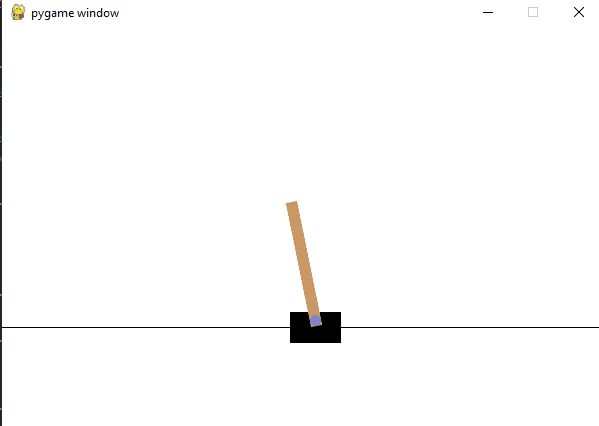
\includegraphics{cartpole_files/image.png}
\caption{image.png}
\end{figure}

    Como esta asignado un punto por segundo, los segundos que dure tiene que
coincidir con la recompensa dada

    \begin{tcolorbox}[breakable, size=fbox, boxrule=1pt, pad at break*=1mm,colback=white, colframe=black]
\prompt{In}{incolor}{11}{\boxspacing}
\begin{Verbatim}[commandchars=\\\{\}]
\PY{k+kn}{from} \PY{n+nn}{IPython}\PY{n+nn}{.}\PY{n+nn}{display} \PY{k+kn}{import} \PY{n}{display}

\PY{c+c1}{\PYZsh{} recompensas en cada jugada}
\PY{n}{display}\PY{p}{(}\PY{n}{tiempos\PYZus{}recompensas}\PY{o}{.}\PY{n}{style}\PY{o}{.}\PY{n}{hide}\PY{p}{(}\PY{n}{axis}\PY{o}{=}\PY{l+s+s2}{\PYZdq{}}\PY{l+s+s2}{index}\PY{l+s+s2}{\PYZdq{}}\PY{p}{)}\PY{o}{.}\PY{n}{set\PYZus{}properties}\PY{p}{(}\PY{o}{*}\PY{o}{*}\PY{p}{\PYZob{}}\PY{l+s+s1}{\PYZsq{}}\PY{l+s+s1}{text\PYZhy{}align}\PY{l+s+s1}{\PYZsq{}}\PY{p}{:} \PY{l+s+s1}{\PYZsq{}}\PY{l+s+s1}{center}\PY{l+s+s1}{\PYZsq{}}\PY{p}{\PYZcb{}}\PY{p}{)}\PY{o}{.}\PY{n}{format}\PY{p}{(}\PY{l+s+s2}{\PYZdq{}}\PY{l+s+si}{\PYZob{}:.2f\PYZcb{}}\PY{l+s+s2}{\PYZdq{}}\PY{p}{)}\PY{p}{)}
\end{Verbatim}
\end{tcolorbox}

\begin{tcolorbox}[breakable, size=fbox, boxrule=1pt, pad at break*=1mm,colback=cellbackground, colframe=cellborder]
    \prompt{Out}{outcolor}{11}{\boxspacing} 
    \centering    
    \begin{tabular}{|c|c|}
            \hline
            Tiempos (s) & Recompensas \\
            \hline
            61.00 & 61.00 \\
            40.00 & 40.00 \\
            38.00 & 38.00 \\
            64.00 & 64.00 \\
            77.00 & 77.00 \\
            30.00 & 30.00 \\
            28.00 & 28.00 \\
            79.00 & 79.00 \\
            29.00 & 29.00 \\
            30.00 & 30.00 \\
            23.00 & 23.00 \\
            58.00 & 58.00 \\
            12.00 & 12.00 \\
            79.00 & 79.00 \\
            40.00 & 40.00 \\
            49.00 & 49.00 \\
            47.00 & 47.00 \\
            35.00 & 35.00 \\
            29.00 & 29.00 \\
            35.00 & 35.00 \\
            \hline
            \end{tabular}
        \end{tcolorbox}


    % Add a bibliography block to the postdoc
    
    
    
\end{document}
